\subsection{Oprava DPS}
    \subsubsection{Oprava vodivého motivu}
        V případě poškozené pájecí plošky a nebo jiné části vodivého motivu je potřeba v prvním kroku danou plošku odebrat. K nahrazení se používá panel s náhradními ploškami, ze kterých je vybrána ploška odpovídající velikosti. V rozporu s návodem k úloze \cite{zadani} jsme nepoužili k připevnění nové plošky epoxidové lepidlo, ale UV světlem vytvrditelnou nepájivou masku. Z naší strany je v tuto metodu drobná pochybnost, neboť nám není jasné, jak dojde k vytvrzení masky pod pájecí ploškou, kam UV světlo neproniklo, ale zřejmě je i tato metoda funkční a o něco rychlejší, než použití dvousložkového epoxidu.

        Po uchycení je potřeba plošku připájet, k tomu jsme využili mikropájku s hrotem. Po pájení je vhodné zkontrolovat multimetrem vodivost nově vytvořeného spoje, což v našem případě dopadlo bez problému. Poté následuje oprava nepájivé masky v místech, kde musela nýt odebrána, aby mohlo dojít ke spojení staré a nové vodivé cesty. Jak probíhá obnovení nepájivé masky je uvedeno v další sekci. 

        \begin{figure}[h!]
            \centering
            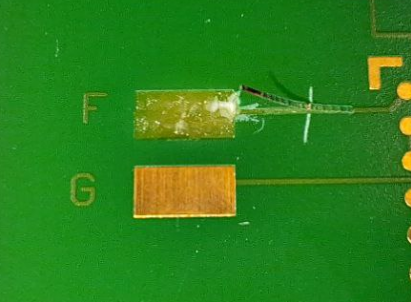
\includegraphics[width=0.6\textwidth]{img/ploska-pred.png}
            \caption{Chybějící pajecí ploška před opravou.}
            \label{fig:obr-ploska-pred-png}
        \end{figure}
        
        \begin{figure}[h!]
            \centering
            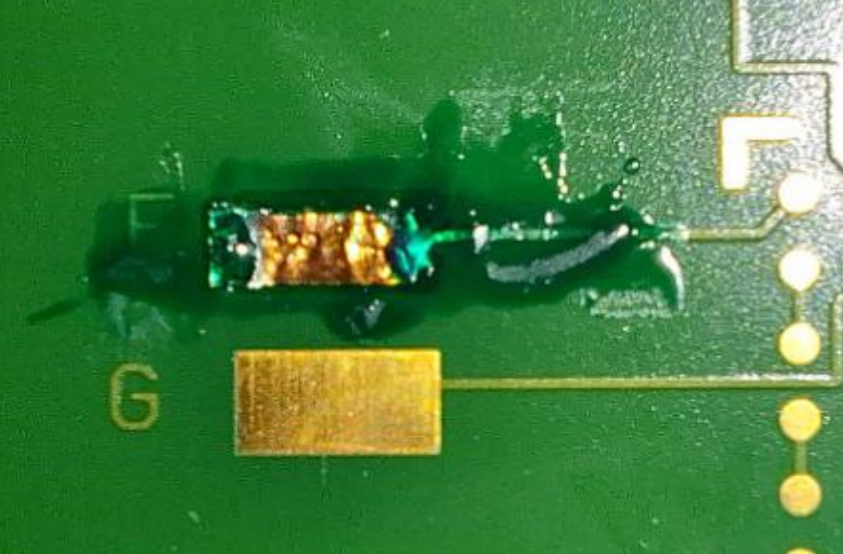
\includegraphics[width=0.6\textwidth]{img/ploska-po.png}
            \caption{Nová pájecí ploška upevněná po připájení a překrytí kontaktu nepájivou maskou.}
            \label{fig:obr-ploska-po-png}
        \end{figure}

    \subsubsection{Oprava nepájivé masky}
        Oprava nepájivé masky je nutná obvykle při fyzickém poškození DPS, kdy dojde k porušení této vrstvy v místě vodivého motivu, což vede k nežádoucímu snížení elektrické pevnosti a zvýšenému riziku zkratu. Také je potřeba tuto opravu provést jako následující po jiné opravě, například výměně poškozené pájecí plošky, kdy je v rámci opravy nutné část původní nepájivé masky odebrat.  

        Pokud je cílem opraváře dosažení vizuálně pěkného výsledku, je vhodným krokem odtranění části nepájivé masky sousedící s poškozeným místem a vytvoření tak symetrického geometrického tvaru. Následně je možné také za pomocí lepicí pásky ohraničit tuto oblast (technika vypůjčena z oblasti malířství). Toto ale nebylo naším cílem, proto byl tento jinak velmi užitečný krok přeskočen.

        Nezbytným dalším krokem je nanesení nové nepájivé masky (UV \textit{LaTeX nechce umět čínské znaky}), to bylo provedeno některým z nástrojů nacházejících se na pracovním stole, nejvhodnějším by byl ovšem bezpochyby štětec. Cílem bylo vytvoření co nejvíce homogenní a hladké vrstvy na vymezené opravované oblasti. 
       